%
% Modified by Megan Patnott
% Last Change: Jan 18, 2013
%
%%%%%%%%%%%%%%%%%%%%%%%%%%%%%%%%%%%%%%%%%%%%%%%%%%%%%%%%%%%%%%%%%%%%%%%%
%
% Modified by Bryce Frentz
% Last Change: 2018
%
%%%%%%%%%%%%%%%%%%%%%%%%%%%%%%%%%%%%%%%%%%%%%%%%%%%%%%%%%%%%%%%%%%%%%%%%
%
% Sample Notre Dame Thesis/Dissertation
% Using Donald Peterson's ndthesis classfile
%
% Written by Jeff Squyres and Don Peterson
%
% Provided by the Information Technology Committee of
%   the Graduate Student Union
%   http://www.gsu.nd.edu/
%
% Nothing in this document is serious except the format.  :-)
%
% If you have any suggestions, comments, questions, please send e-mail
% to: ndthesis@gsu.nd.edu
%
%%%%%%%%%%%%%%%%%%%%%%%%%%%%%%%%%%%%%%%%%%%%%%%%%%%%%%%%%%%%%%%%%%%%%%%%

%
% Chapter 3
%

\chapter{Cross section data Reduction and analysis}
\label{chap: data}

\section{Introduction}

In aggregate, the data taken at both the CASPAR and NSL experiments consists of $\gamma$-ray energy data from the $^{14}$N$\left( p,\gamma \right) ^{15}$O reaction, observed with a single, 130\% HPGe detector placed at $55^{\degree}$ relative to the beam direction. These data were collected for reactions over the combined proton energy range of 270 - 1200 keV. The primary interest of these experiments was monitoring the R/DC$\rightarrow$GS transition and the R/DC$\rightarrow$6.79 MeV + 6.79 MeV$\rightarrow$GS transition sequence. As such, the energies of the concerned photons ranged in energy from $\sim$600 keV up to $\sim$8500 keV. This chapter details the processes by which this data is gathered and turned into an experimental cross section.

\section{Angular corrections}
\label{sec: angularCorrections}

The angular distribution of a cross section, $W$, can be described by

\begin{equation}
W_{\text{exp}} = a_{0} \left(1 + \sum_{i = 1}^{n} a_{i} Q_{i} P_{i} ( \cos (\theta) )    \right)
\end{equation}

\noindent where $a_{i}$ are the angular distribution coefficients, $Q_{i}$ are correction factors due to the finite size of a given detector, and the $P_{i} ( \cos (\theta) )$ are the Legendre polynomials of order $i$. For the conditions of this work, odd numbered terms as well as those of order higher than 2 give negligible contribution to the angular distribution. Therefore, the resulting angular distribution of this reaction is of the form

\begin{equation}
W_{\text{exp}} = a_{0} + a_{2} Q_{2} P_{2} ( \cos (\theta) ).
\end{equation}

Experimentally, to address any effects arising from an angular distribution of this form, the detector was placed at $55^{\degree}$. This is the zero of the 2nd order Legendre polynomial, thereby minimizing any effects on the cross section arising from the detector's angle. Simultaneously, this means that no correction of the data is necessary.


\section{Energy calibration}
\label{sec: energy calibration}

It is important to establish the true relationship between $\gamma$-rays of different energies incident in a detector and the signal they produce during data acquisition. This connection is determined by calibrating the system with $\gamma$-rays of well-known energy from room background, given radioactive sources, like $^{137}$Cs or $^{60}$Co, and well-studied nuclear reactions, like $^{27}$Al($p, \gamma$)$^{28}$Si. The reactions are also used in calibration because no natural sources of radioactivity provide $\gamma$'s with energy higher than 3.6 MeV, whereas the $^{27}$Al($p, \gamma$)$^{28}$Si reaction provides $\gamma$ ray energies up to 10.7 MeV, ensuring that the detector is well calibrated over the entire energy range for $\gamma$'s that will be seen in the $^{14}$N$\left( p,\gamma \right) ^{15}$O reaction. The exact relationship between the the channel number in the acquisition system analog-to-digital converter (ADC) and the incident photon energy, $E_{\gamma}$, is characterized by the standard linear relationship

\begin{equation}
E_{\gamma} = m \times \text{Channel} + b
\end{equation}

\noindent where $m$ is simply the slope and $b$ the offset of the fit. For a HPGe detector, a linear relationship is sufficient and appropriate to describe the ADC response. However, this process was redone for every phase of the experiment because slightly different gains applied to the ADC's and signal amplifiers provide a different relationship in the electronics. Therefore, despite using the same detector, each phase of the experiment required its own energy calibration, an example of which is shown in Fig.\ \


\begin{figure}
\centering
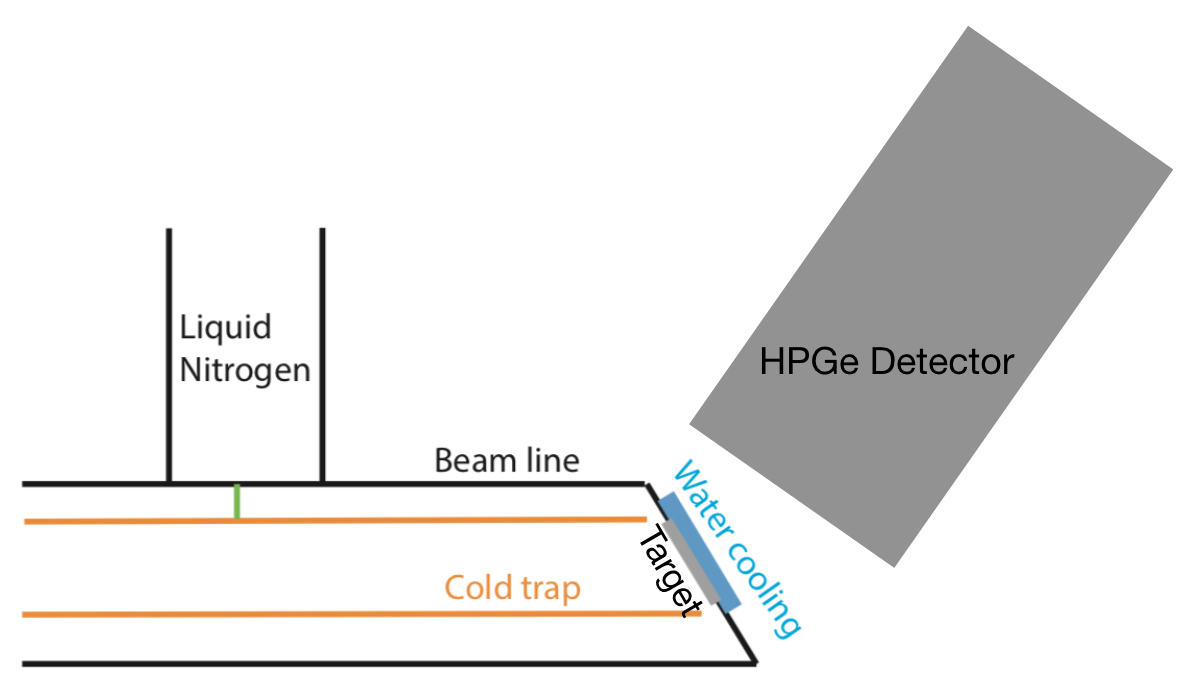
\includegraphics[width=0.8\linewidth]{figures/expSetup.png}
\label{fig: energyCalibration}
\caption{Energy calibration curve for the HPGe detector taken at CASPAR. The calibration incorporated natural background, radioactive sources, and the products from the $^{27}$Al($p, \gamma$)$^{28}$Si reaction. }
\end{figure}




\section{Efficiency}
\label{sec: efficiency}

For this experiment, both the total efficiency, $\eta^{tot}$, and the full-energy peak (FEP) efficiency, $\eta^{fep}$, were required. The total efficiency is the probability that the $\gamma$ ray enters and deposits any amount of energy within the detector, while, on the other hand, the FEP efficiency is the probability that the full energy of an emitted $\gamma$ ray will be deposited within the detector. As both efficiency types are dependent on the physical geometry of the system, they are determined for each experimental setup in turn. 

\subsection{Total efficiency}

The total efficiency of a detector / source geometry is the probability that a given photon from the source will enter and deposit any amount of energy within the detector. For extremely simple geometries, the total efficiency can be calculated following the approach laid out in Debertin and Helmer cite{DebertinHelmerBook},

\begin{equation}
\eta^{tot} = \dfrac{1}{4\pi} \int \left(1 - e^{-\mu x} \right) d\Omega
\end{equation}

\noindent where $\mu$ is the energy and absorber dependent attenuation coefficient, x is the position from the detector face, and the integration takes place over the solid angle of the detector from the front to the back. This formulation makes it abundantly clear that $\eta^{tot}$ is so highly dependent on the geometry of the setup. 

However, in practice, there is no analytic formulation of the total efficiency because one needs to account for any potential scattering of $\gamma$-rays off of any surrounding material, like the shielding or target chamber, for example. Additionally, when measuring the total efficiency for a given setup, the presence of multiple decays from physical sources provides additional complications. Therefore, most commonly the total efficiency is determined using single-line radioactive sources, like $^{137}$Cs. In this case, when accounting for the ever-present background, the total efficiency is the total number of counts in a spectrum divided by the total number of decays occurring during the measurement time, which can be easily calculated with the radioactive decay law

\begin{equation}
N(t) = N_{0} e^{- \lambda t} \hfill A(t) = A_{0} e^{- \lambda t},
\end{equation}

\noindent where $N(t)$ is the number of nuclei remaining after time $t$, $N_{0}$ is the initial number of radioactive nuclei, $\lambda$ is the radioactive decay constant for a given nucleus, $A(t)$ is the activity of the source at time $t$ compared to the activity at time $t=0$ of $A_{0}$. The decay constant, $\lambda$, can be calculated from either the nuclear lifetime, $\tau$, or the decay half-life, $t_{1/2}$, as

\begin{equation}
\lambda = \dfrac{1}{\tau} \hfill \lambda = \dfrac{\text{ln}(2)}{t_{1/2}}.
\end{equation}

\noindent This is how the total efficiency for the detector systems was determined at 662 keV, the $\gamma$ energy from the decay of $^{137}$Cs.



\begin{figure}
\centering
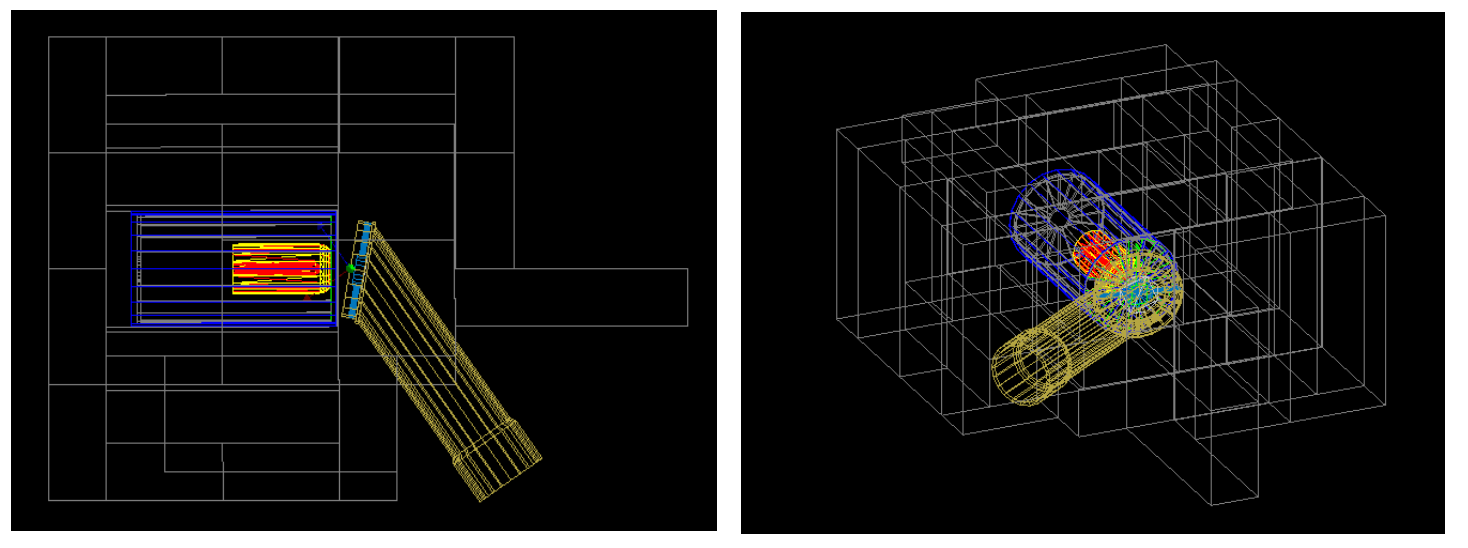
\includegraphics[width=\linewidth]{figures/shieldingSimulation.png}
\label{fig: simulatedSetup}
\caption{Simulation of the experimental setup at CASPAR, including the target chamber (in gold), water cooling (in light blue), HPGe detector (in dark blue), and lead bricks for shielding (in gray). Both pictures are of the same experimental setup from different angles to convey the layout. Simulating this setup is necessary to determine the total efficiency of the experimental setup. In this determination, a single-line $\gamma$ source is placed at the target location and its decays simulated for a variety of energies, allowing a determination of the total efficiency at each.}
\end{figure}


\begin{figure}
\centering
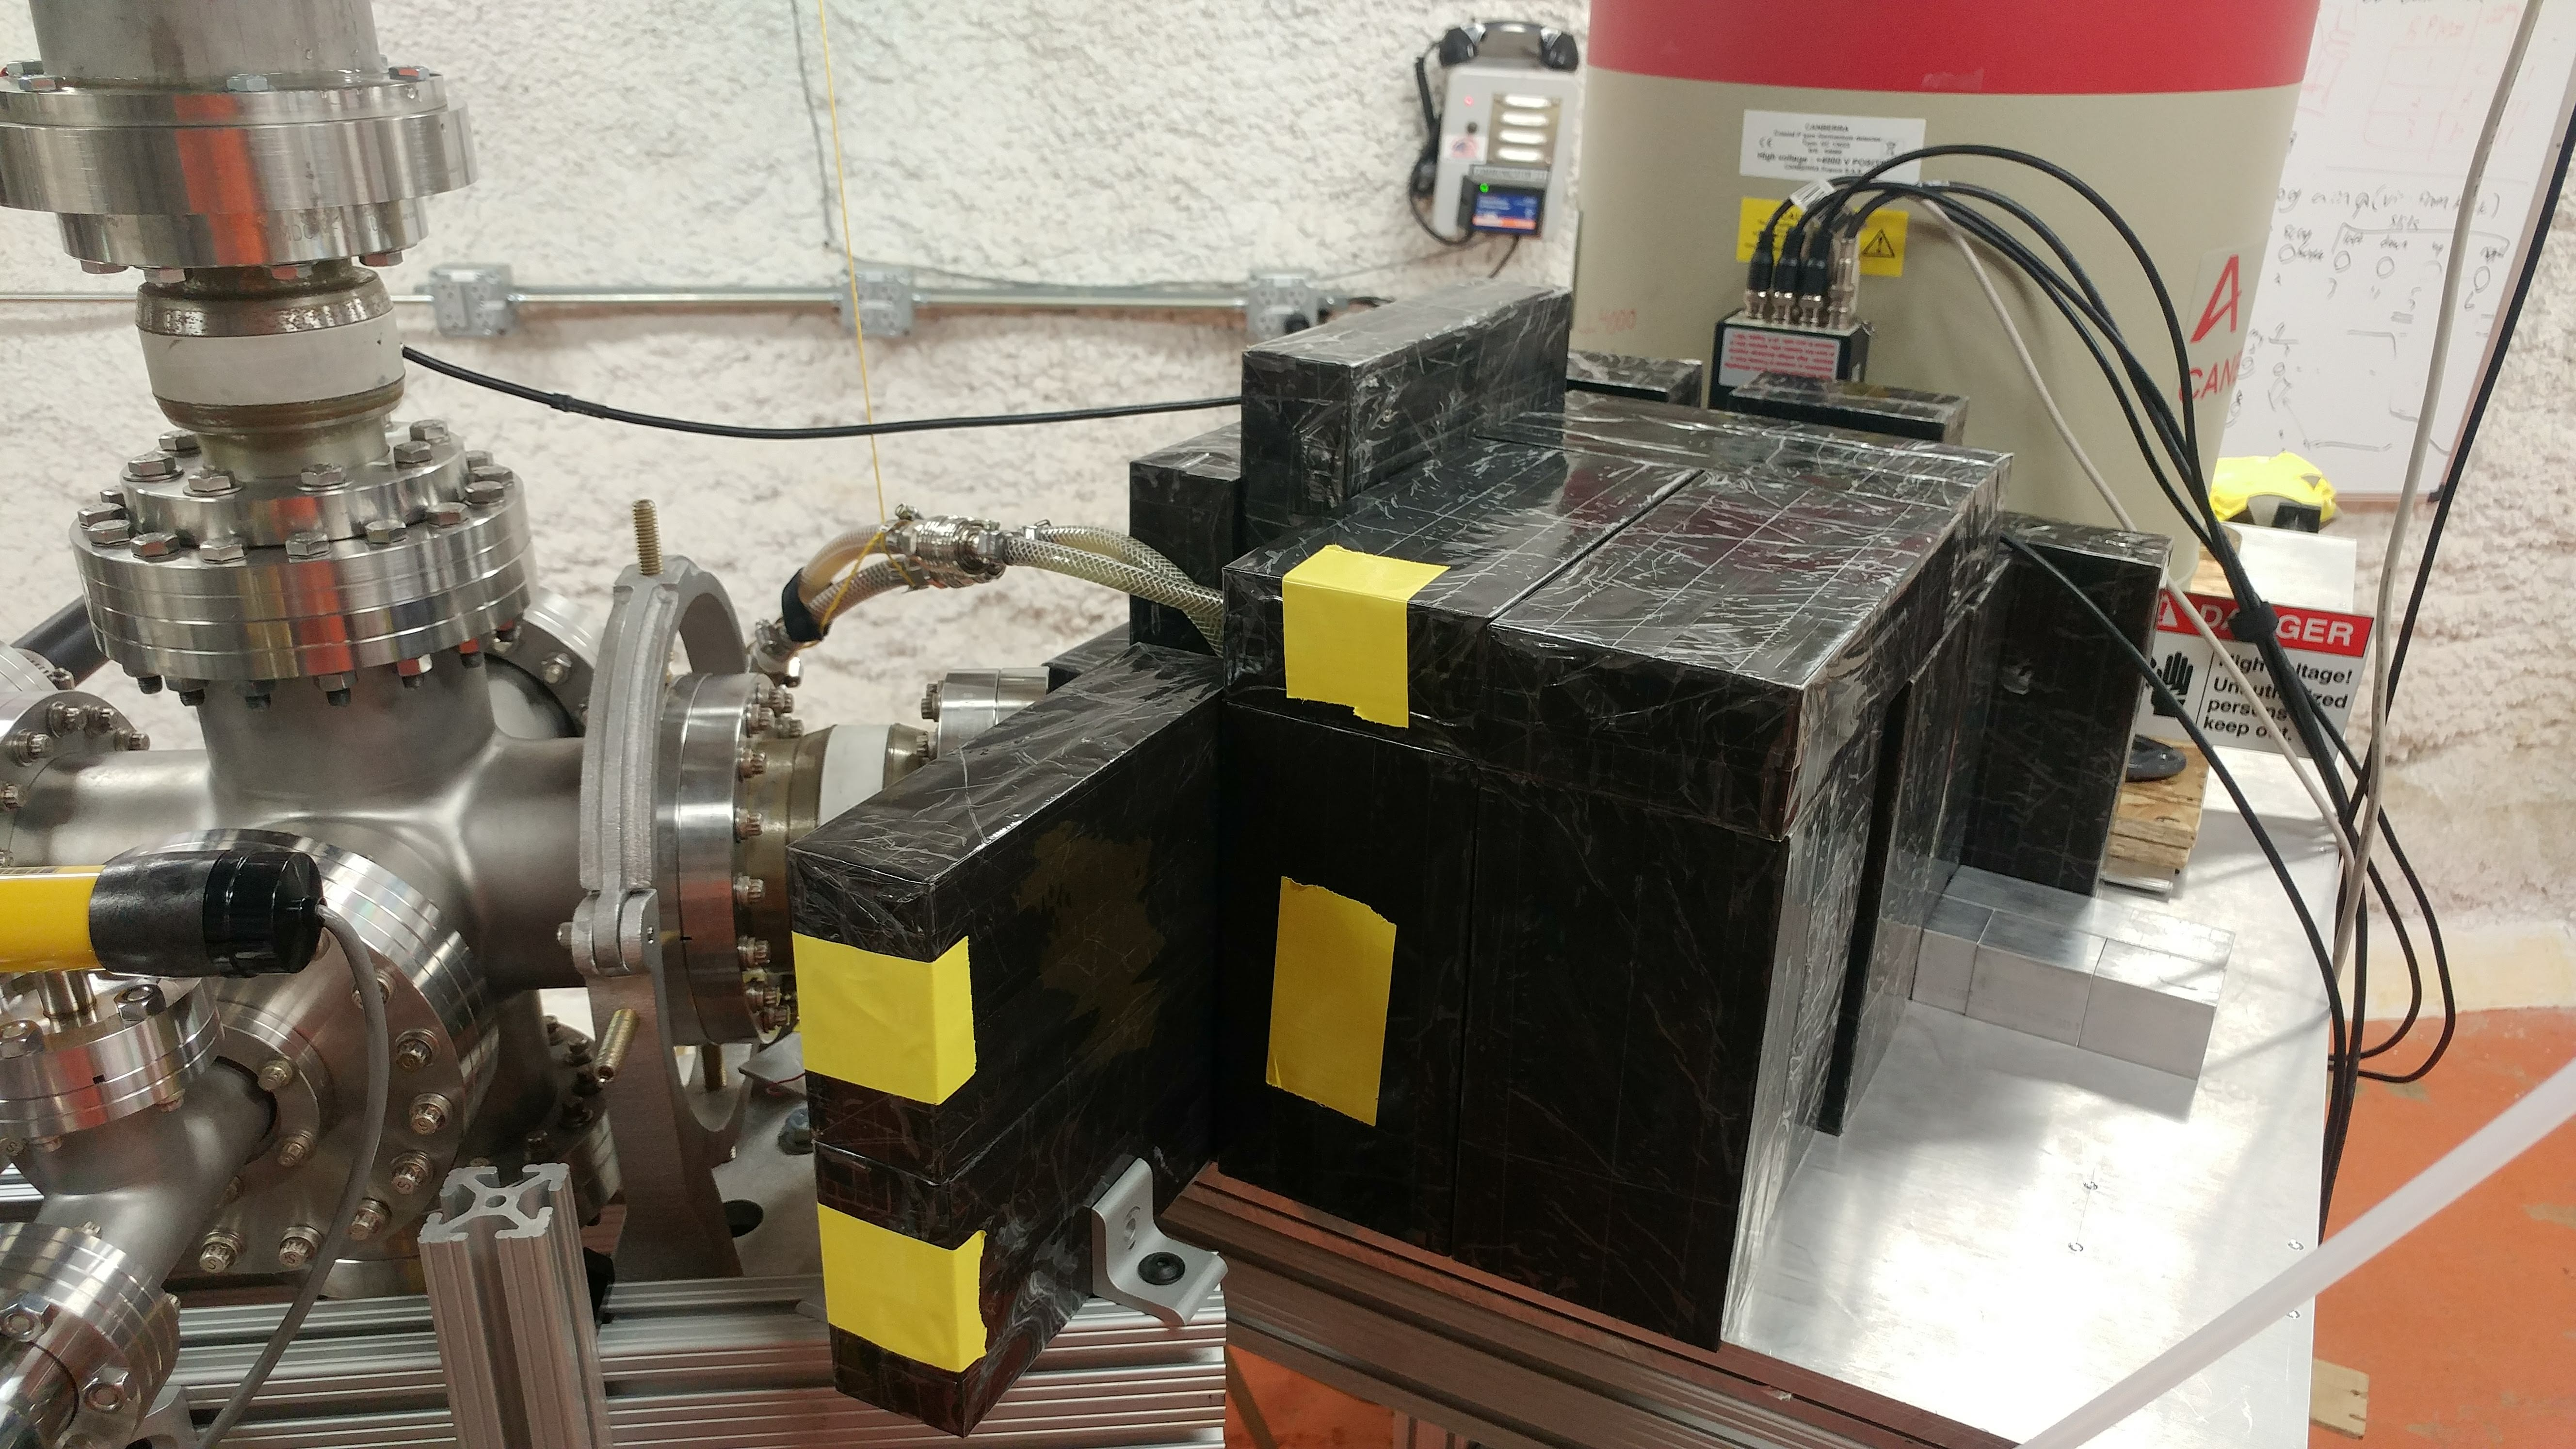
\includegraphics[width=0.8\linewidth]{figures/shieldingPicture.jpg}
\label{fig: actualSetup}
\caption{A picture of the experimental setup at CASPAR, showing the lead shielding around the detector and target chamber. This figure is provided for comparison to the simulated setup to prove its accuracy. }
\end{figure} 

To extend $\eta^{tot}$ to the whole range of energies relevant to the experiments, the experimental setup (including the target chamber, water cooling, and shielding) was built and simulated in Geant4 \cite{Agostinelli2003}, an example of the simulation for the CASPAR setup is shown in Fig.\ \ref{fig: simulatedSetup} where the actual setup is given in Fig.\ \ref{fig: actualSetup} for comparison. Then, a single-emission source was placed at the target location and simulated 10,000,000 decays, recording the deposited energy inside the detector. The energy of the source was changed and simulated at energies of 662, 1300, 2000, 3000, 4000, 6000, 7000, 8000, and 10000 keV to cover the entire range of $\gamma$ ray energies present in the $^{14}$N$\left( p,\gamma \right) ^{15}$O reaction. For each of the different decay energies, the spectrum of recorded events in the detector was analyzed in the exact same way as the actual $^{137}$Cs data to produce the total efficiency at each energy. This simulated data was used in conjunction with the measured $^{137}$Cs total efficiency data point to determine an accurate curve of the total efficiency across all experimentally relevant energies, shown in Fig.\ \ref{fig: totalEfficiency}.

\begin{figure}
\centering
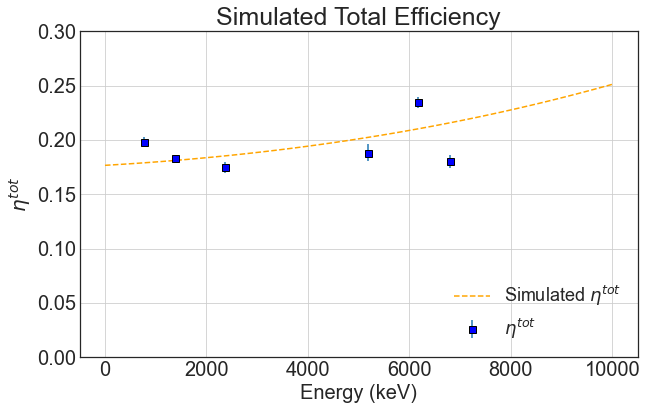
\includegraphics[width=\linewidth]{figures/totalEfficiency.png}
\label{fig: totalEfficiency}
\caption{The total efficiency of the HPGe in the CASPAR setup across all relevant energies. The points from the Geant4 simulation are taken raw without scaling, showing the efficacy of this technique and accuracy of the simulation.  }
\end{figure}



\subsection{Full energy peak efficiency}


\section{Summing corrections}
\label{sec: summing}

\section{Target characterization}
\label{sec: target}

\section{Cross-section determination}
\label{sec: cross-section}





% % uncomment the following lines,
% if using chapter-wise bibliography
%
% \bibliographystyle{ndnatbib}
% \bibliography{example}
